\chapter{Preventivo}\label{Prev}
\begin{flushleft}
Di seguito viene riportato il preventivo per il progetto \textit{MegAlexa$_{G}$}; esso si divide, per ogni periodo, in:
\begin{itemize}
	\item \textbf{Prospetto orario:} presenta la distribuzione oraria e la suddivisione nei ruoli per ogni membro del gruppo \textit{ZeroSeven$_{G}$};
	\item \textbf{Prospetto economico:} presenta le ore di impegno calcolate per i ruoli coinvolti ed il rispettivo costo.
\end{itemize}
La suddivisione oraria viene svolta avendo come riferimento le seguenti regole:
\begin{itemize}
	\item Ogni membro del gruppo deve coprire ogni ruolo almeno una volta durante il ciclo di sviluppo del prodotto;
	\item Il totale delle ore di lavoro deve essere equamente distribuito tra i membri;
	\item Non ci devono essere conflitti di interesse in cui un \textit{Verificatore} debba controllare il proprio lavoro.
\end{itemize}
Le sigle utilizzate per i vari ruoli saranno:
\begin{itemize}
	\item \textbf{Re:} \textit{Responsabile di Progetto};
	\item \textbf{Am:} \textit{Amministratore};
	\item \textbf{An:} \textit{Analista};
	\item \textbf{Pt:} \textit{Progettista};
	\item \textbf{Pr:} \textit{Programmatore};
	\item \textbf{Ve:} \textit{Verificatore}.
\end{itemize}
Per il preventivo si tiene conto che il periodo di Analisi è considerato di investimento del gruppo e non a carico dei committente, per cui le ore di impegno svolte durante questo periodo non saranno conteggiate nelle ore totali da retribuire.
\end{flushleft}
\newpage
\section{Analisi }
\subsection{Prospetto orario}
Il prospetto orario per il periodo di Analisi è illustrato nella seguente tabella:

\begin{table}[ht]
	\begin{center}
		\rowcolors{1}{}{lightgray}
		\begin{tabular}{cccccccccccc}
			\rowcolor{coolblack}
			\hline 
			& \textcolor{white}{Nome} & \textcolor{white}{Re} & \textcolor{white}{Am} & \textcolor{white}{An} & \textcolor{white}{Pt} &\textcolor{white}{Pr} & \textcolor{white}{Ve} & \textcolor{white}{Totale} \\
			\hline
			
			&Mirko Franco          & 10 & - & 9 & - & - & 5 &24  \\
			&Bianca Andreea Ciuche        & -  & 6 & 10 & - & - & 8 & 24 \\
			&Stefano Zanatta     & 12& 8 & 4 & - & - & - & 24 \\
			&Andrea Deidda       &  -& 9 & 8 & - & - & 7 & 24 \\
			&Ludovico Brocca    & -& 4 & 9 & - & - & 11 & 24 \\
			&Matteo Depascale  & -& 6& 10 & - & - & 8 & 24 \\
			&Gian Marco Bratzu & -& 6 & 8 & - & - & 10 & 24 \\
			\hline
			&\textbf{Ore totali ruolo} & 22 & 39 & 58 & - & - & 49 & 168 \\
		\end{tabular}
		\caption{Prospetto orario nel periodo di Analisi}
	\end{center}
\end{table}

Il seguente grafico rappresenta la suddivisione oraria dei ruoli all'interno del gruppo:
\begin{figure}[!ht]
	\begin{center}
		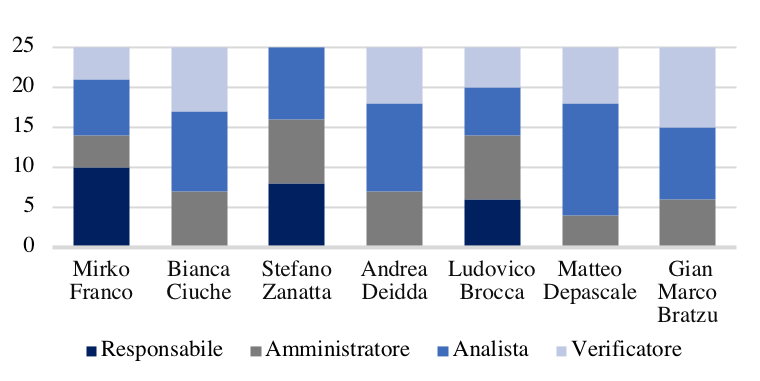
\includegraphics[scale=0.90]{images/grafoProspettoOrario.png}
		\caption{Grafico prospetto orario nel periodo di Analisi}
	\end{center}
\end{figure}

\subsection{Prospetto economico}
Il prospetto economico per il periodo di Analisi è illustrato nella seguente tabella.
Le spese non sono a carico del committente.

\begin{table}[ht]
	\begin{center}
		\rowcolors{1}{}{lightgray}
			\begin{tabular}{cccccc}
			\rowcolor{coolblack}
			\hline
			&\textcolor{white}{Ruolo}&	\textcolor{white}{Ore} &\textcolor{white}{Costo(\euro)} \\
			\hline
			&Responsabile           &22& 660  \\
			&Amministratore        & 39& 780 \\
			&Analista                   & 58& 1.450 \\
			&Progettista              &  -& - \\
			&Programmatore       & - & -  \\
			&Verificatore             & 49 & 735 \\
			\hline
			&\textbf{Ore totali}    &168& 3.625 \\
		\end{tabular}
		\caption{Prospetto economico nel periodo di Analisi}
	\end{center}
\end{table}

La raffigurazione grafica del peso di ogni ruolo sul costo totale è così rappresentata:
\begin{figure}[!ht]
	\centering
	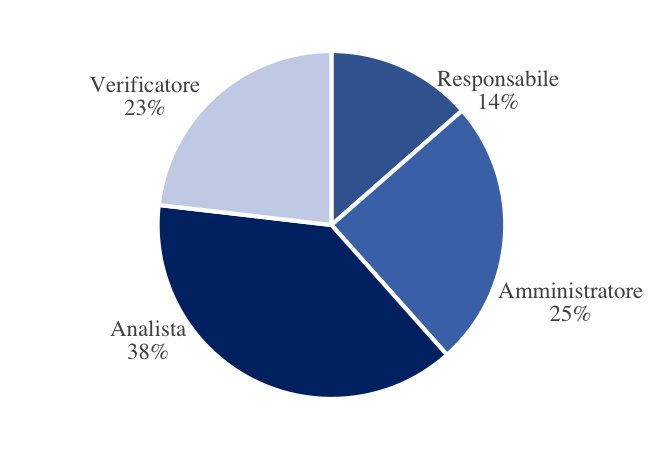
\includegraphics{images/grafoProspettoEconomico.png}
	\caption{Grafico prospetto economico nel periodo di Analisi }
\end{figure}

\newpage

\section{Revisione Analisi}
\subsection{Prospetto orario}
Il prospetto orario per il periodo di Revisione Analisi è illustrato nella seguente tabella:

\begin{table}[ht]
	\begin{center}
		\rowcolors{1}{}{lightgray}
		\begin{tabular}{cccccccccccc}
			\rowcolor{coolblack}
			\hline 
			& \textcolor{white}{Nome} & \textcolor{white}{Re} & \textcolor{white}{Am} & \textcolor{white}{An} & \textcolor{white}{Pt} &\textcolor{white}{Pr} & \textcolor{white}{Ve} & \textcolor{white}{Totale} \\
			\hline
			
			&Mirko Franco          & - & 3 & - & - & - & 2 &5  \\
			&Bianca Andreea Ciuche        & 5  & - & - & - & - & - & 5 \\
			&Stefano Zanatta     & -& - & 2 & - & - & 3&5 \\
			&Andrea Deidda       &  -& - & 2 & - & - & 3 &5 \\
			&Ludovico Brocca    & -& -& 3 & - & - & 2 & 5 \\
			&Matteo Depascale  & -& 2& -& - & - & 3 & 5 \\
			&Gian Marco Bratzu & -& - & 2 & - & - & 3& 5 \\
			\hline
			&\textbf{Ore totali ruolo} & 5 & 5 & 9 & - & - & 16 & 35 \\
		\end{tabular}
		\caption{Prospetto orario nel periodo di Revisione Analisi}
	\end{center}
\end{table}

Il seguente grafico rappresenta la suddivisione oraria dei ruoli all'interno del gruppo:
\begin{figure}[!ht]
	\begin{center}
		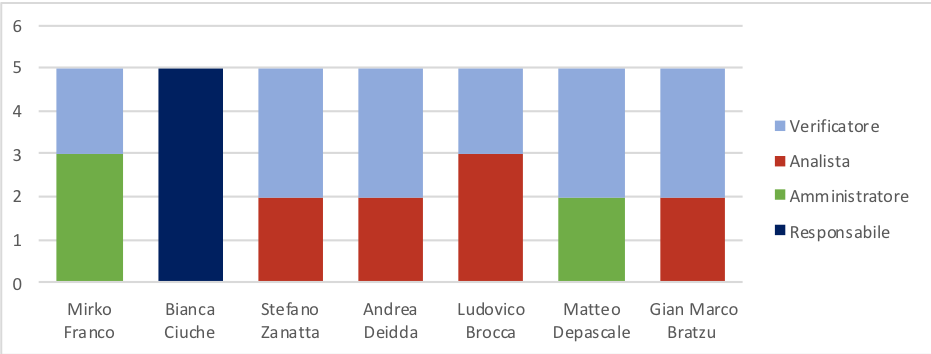
\includegraphics{images/grafoProspettoOrarioDett.png}
		\caption{Grafico prospetto orario nel periodo di Revisione Analisi }
	\end{center}
\end{figure}
\newpage
\subsection{Prospetto economico}
Il prospetto economico per il periodo di Revisione Analisi è illustrato nella seguente tabella.
Le spese sono a carico del committente.
\begin{table}[ht]
	\begin{center}
		\rowcolors{1}{}{lightgray}
		\begin{tabular}{cccccc}
			\rowcolor{coolblack}
			\hline
			&\textcolor{white}{Ruolo}&	\textcolor{white}{Ore} &\textcolor{white}{Costo(\euro)} \\
			\hline
			&Responsabile           &5&150  \\
			&Amministratore        & 5& 100 \\
			&Analista                   & 9& 225 \\
			&Progettista              &  -& - \\
			&Programmatore       & - & -  \\
			&Verificatore             & 16 & 240 \\
			\hline
			&\textbf{Ore totali}    &35& 715\\
		\end{tabular}
		\caption{Prospetto economico nel periodo di Revisione Analisi }
	\end{center}
\end{table}

La raffigurazione grafica del peso di ogni ruolo sul costo totale è così rappresentata: 
\begin{figure}[!ht]
	\begin{center}
		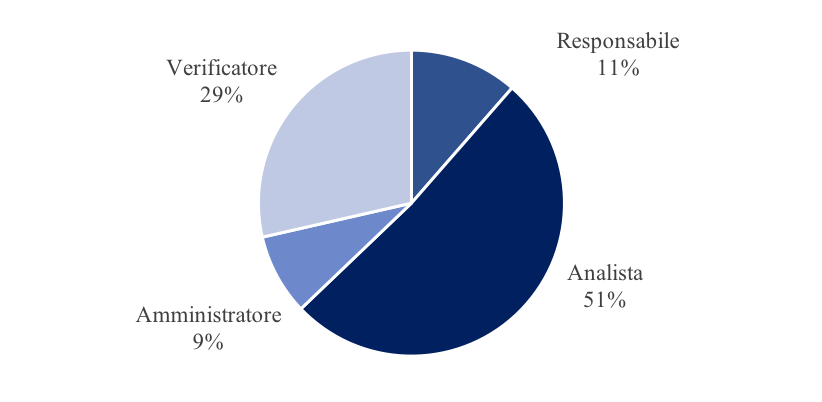
\includegraphics{images/grafoProspettoEconomicoDett.png}
		\caption{Grafico prospetto economico nel periodo di Revisione Analisi}
	\end{center}
\end{figure}

\newpage

\section{Progettazione della base tecnologica}
\subsection{Prospetto orario}
Il prospetto orario durante il periodo di Progettazione della Base Tecnologica è illustrato nella seguente tabella:

\begin{table}[ht]
	\begin{center}
		\rowcolors{1}{}{lightgray}
		\begin{tabular}{ccccccccc}
			\rowcolor{coolblack}
			\hline
			& \textcolor{white}{Nome} & \textcolor{white}{Re} & \textcolor{white}{Am} & \textcolor{white}{An} & \textcolor{white}{Pt} &\textcolor{white}{Pr} & \textcolor{white}{Ve} & \textcolor{white}{Totale} \\
			\hline
			&Mirko Franco & - & - & 9 & 10 & 6 & - & 25  \\
			&Bianca Andreea Ciuche & -& - & 6 & 8 & - & 11 & 25 \\
			&Stefano Zanatta &- & - & - & 24 &  & - & 24 \\
			&Andrea Deidda &  -& - & - & 12 & 4 & 11 & 27 \\
			&Ludovico Brocca & -& 5 & - & 16 & 5 & - & 26 \\
			&Matteo Depascale & -& - & - & 12 & - & 12 & 24 \\
			&Gian Marco Bratzu & 7& - & - & 19 & - & - & 26 \\
			\hline
			&\textbf{Ore totali ruolo} & 7 & 5 & 15 & 101 & 15 & 34 & 177 \\
		\end{tabular}
		\caption{Prospetto orario nel periodo di Progettazione della base tecnologica}
	\end{center}
\end{table}

Il seguente grafico rappresenta la suddivisione oraria dei ruoli all'interno del gruppo:
\begin{figure}[!ht]
	\begin{center}
		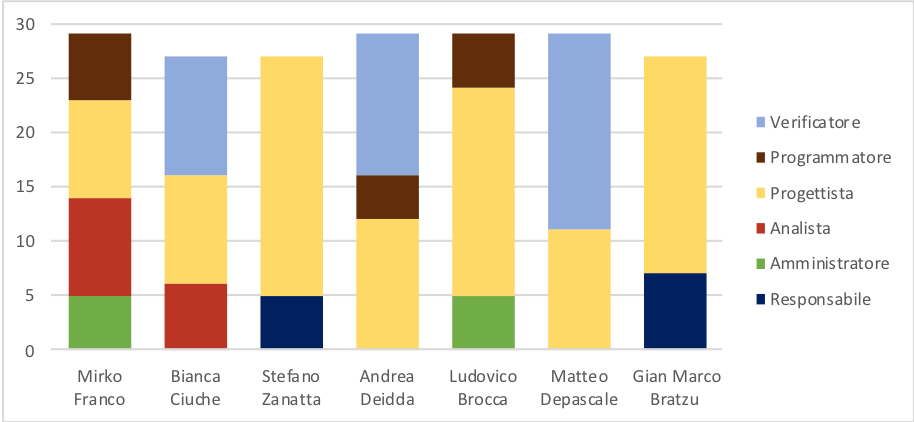
\includegraphics[scale=0.85]{images/grafoProgettazioneTecnologica.png}
		\caption{Grafico prospetto orario nel periodo di Progettazione della Base Tecnologica}
	\end{center}
\end{figure}
\newpage
\subsection{Prospetto economico}
Il prospetto economico per il periodo di Progettazione della base tecnologica è illustrato nella seguente tabella:

\begin{table}[ht]
	\begin{center}
		\rowcolors{1}{}{lightgray}
		\begin{tabular}{cccccc}
			\rowcolor{coolblack}
			\hline
			&\textcolor{white}{Ruolo}&	\textcolor{white}{Ore} &\textcolor{white}{Costo(\euro)} \\
			\hline
			&Responsabile           &7&210 \\
			&Amministratore        & 5& 100 \\
			&Analista                   & 15& 375 \\
			&Progettista              &  101& 2.222\\
			&Programmatore       & 15& 225 \\
			&Verificatore             & 34& 510 \\
			\hline
			&\textbf{Ore totali}    &177&3.642\\
		\end{tabular}
		\caption{Prospetto economico nel periodo di Progettazione della base tecnologica}
	\end{center}
\end{table}


La raffigurazione grafica del peso di ogni ruolo sul costo totale è così rappresentata:
\begin{figure}[!ht]
	\begin{center}
		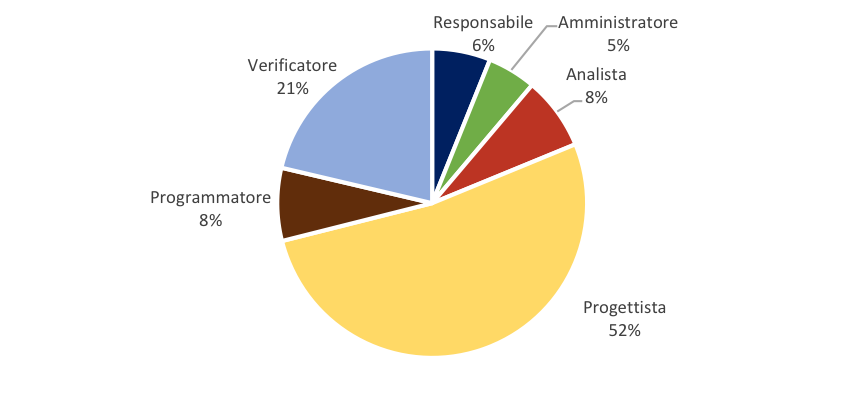
\includegraphics[scale=0.90]{images/grafoProgettazioneTecnologicaEuro.png}
		\caption{Grafico prospetto economico nel periodo di Progettazione della Base Tecnologica}
	\end{center}
\end{figure}
\newpage
\section{Progettazione di Dettaglio e Codifica}
\subsection{Prospetto orario}
Il prospetto orario durante il periodo di Progettazione di Dettaglio e Codifica è illustrato nella seguente tabella:

\begin{table}[ht]
	\begin{center}
		\rowcolors{1}{}{lightgray}
		\begin{tabular}{ccccccccc}
			\rowcolor{coolblack}
			\hline
			& \textcolor{white}{Nome} & \textcolor{white}{Re} & \textcolor{white}{Am} & \textcolor{white}{An} & \textcolor{white}{Pt} &\textcolor{white}{Pr} & \textcolor{white}{Ve} & \textcolor{white}{Totale} \\
			\hline
			&Mirko Franco & - & - & - & 9 & 21 & 20 & 50  \\
			&Bianca Andreea Ciuche & -& 6& - & 16 & 21 & 8 & 51 \\
			&Stefano Zanatta & - & - & 4 & 14 & 22 & 10 & 50 \\
			&Andrea Deidda &  -& - & 7 & 23 & 20 & - & 50 \\
			&Ludovico Brocca & 8& - & - & 14 & 19 & 10 & 51 \\
			&Matteo Depascale & -& 6& - & 19 & 12 & 13 & 50 \\
			&Gian Marco Bratzu & -& - & - & 22 & 19 & 10 & 51 \\
			\hline
			&\textbf{Ore totali ruolo} & 8 & 12 & 11 & 117 & 134 & 71 & 353 \\
		\end{tabular}
	\caption{Prospetto orario nel periodo di Progettazione di Dettaglio e Codifica}
	\end{center}
\end{table}

Il seguente grafico mostra una rappresentazione visiva della suddivisione oraria dei ruoli all'interno del gruppo:
\begin{figure}[!ht]
	\begin{center}
		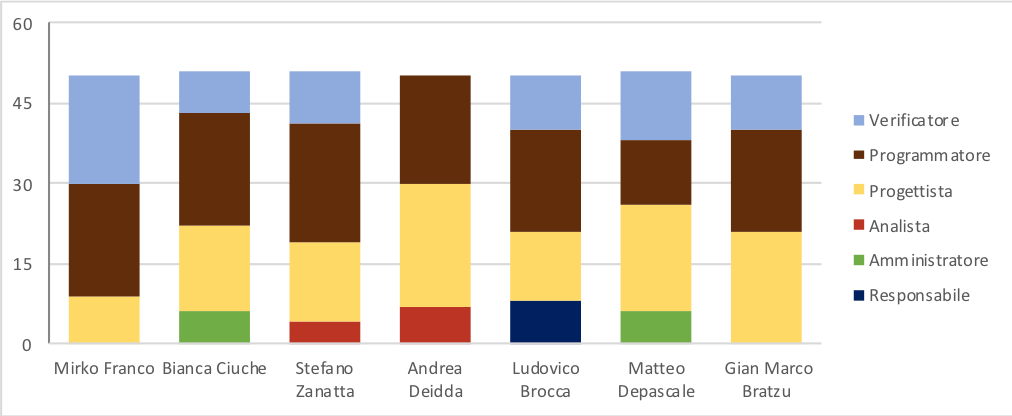
\includegraphics[scale=0.80]{images/grafoProgettazioneDettaglioCodifica.png}
		\caption{Grafico prospetto orario nel periodo di Progettazione di Dettaglio e Codifica}
	\end{center}
\end{figure}

\subsection{Prospetto economico}
Il prospetto economico durante il periodo di Progettazione di Dettaglio e Codifica è illustrato nella seguente tabella:

\begin{table}[ht]
	\begin{center}
		\rowcolors{1}{}{lightgray}
		\begin{tabular}{cccccc}
			\rowcolor{coolblack}
			\hline
			&\textcolor{white}{Ruolo}&	\textcolor{white}{Ore} &\textcolor{white}{Costo(\euro)} \\
			\hline
			&Responsabile           &8&240\\
			&Amministratore        & 12& 240 \\
			&Analista                   & 11& 275 \\
			&Progettista              &  117& 2.574\\
			&Programmatore       & 134& 2.010 \\
			&Verificatore             & 71& 1.065 \\
			\hline
			&\textbf{Ore totali}    &353&6.404\\
		\end{tabular}
		\caption{Prospetto economico nel periodo di Progettazione di Dettaglio e Codifica}
	\end{center}
\end{table}

La raffigurazione grafica del peso di ogni ruolo sul costo totale è così rappresentata:

\begin{figure}[!ht]
	\begin{center}
		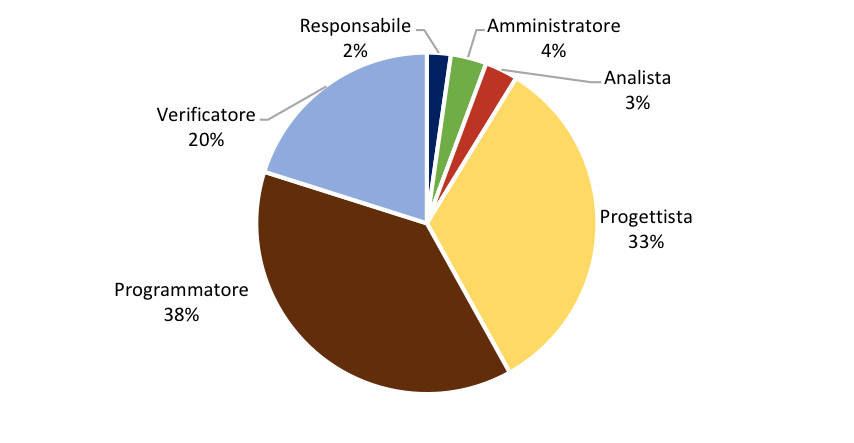
\includegraphics{images/grafoProgettazioneDettaglioCodificaEuro.png}
		\caption{Grafico prospetto economico nel periodo di Progettazione di Dettaglio e Codifica}
	\end{center}
\end{figure}

\newpage
\section{Validazione e Collaudo}
\subsection{Prospetto orario}
Il prospetto orario durante il periodo di Validazione e Collaudo è illustrato nella seguente tabella:

\begin{table}[ht]
	\begin{center}
		\rowcolors{1}{}{lightgray}
		\begin{tabular}{ccccccccc}
			\rowcolor{coolblack}
			\hline
			& \textcolor{white}{Nome} & \textcolor{white}{Re} & \textcolor{white}{Am} & \textcolor{white}{An} & \textcolor{white}{Pt} &\textcolor{white}{Pr} & \textcolor{white}{Ve} & \textcolor{white}{Totale} \\
			\hline
			&Mirko Franco & - & - & 4 & 9& - & 11 & 24  \\
			&Bianca Andreea Ciuche & -& -& - & 12 & - & 11 & 23 \\
			&Stefano Zanatta & - & 8& 4 & - & - & 13 & 25 \\
			&Andrea Deidda &  6& - & - & - & - & 16 & 22 \\
			&Ludovico Brocca & -& 9 & - & - & - & 13 & 22 \\
			&Matteo Depascale & 6& -& 4 & 3& 12& -& 25 \\
			&Gian Marco Bratzu & -& 4 & - & - & 13 & 5 & 22 \\
			\hline
			&\textbf{Ore totali ruolo} & 12& 21 & 12 & 24 & 25 & 69 & 163 \\
		\end{tabular}
		\caption{Prospetto orario nel periodo di Validazione e Collaudo}
	\end{center}
\end{table}

Il seguente grafico mostra una rappresentazione visiva della suddivisione oraria dei ruoli all'interno del gruppo:
\begin{figure}[!ht]
	\begin{center}
		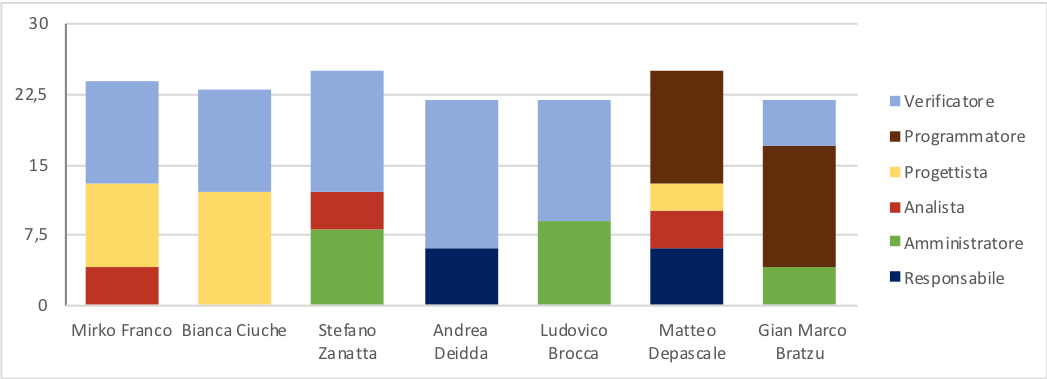
\includegraphics[scale=0.80]{images/grafoValidazioneCollaudo.png}
		\caption{Grafico prospetto orario nel periodo di Validazione e Collaudo}
	\end{center}
\end{figure}

\subsection{Prospetto economico}
Il prospetto economico durante il periodo di Validazione e Collaudo è illustrato nella seguente tabella:

\begin{table}[ht]
	\begin{center}
		\rowcolors{1}{}{lightgray}
		\begin{tabular}{cccccc}
			\rowcolor{coolblack}
			\hline
			&\textcolor{white}{Ruolo}&	\textcolor{white}{Ore} &\textcolor{white}{Costo(\euro)} \\
			\hline
			&Responsabile           &12&360\\
			&Amministratore        & 21& 420 \\
			&Analista                   & 12& 300\\
			&Progettista              &  24& 528\\
			&Programmatore       & 25& 375 \\
			&Verificatore             & 69& 1.035\\
			\hline
			&\textbf{Ore totali}    &163&3.018\\
		\end{tabular}
		\caption{Prospetto economico nel periodo di Validazione e Collaudo}
	\end{center}
\end{table}

La raffigurazione grafica del peso di ogni ruolo sul costo totale è così rappresentata:
\begin{figure}[!ht]
	\begin{center}
		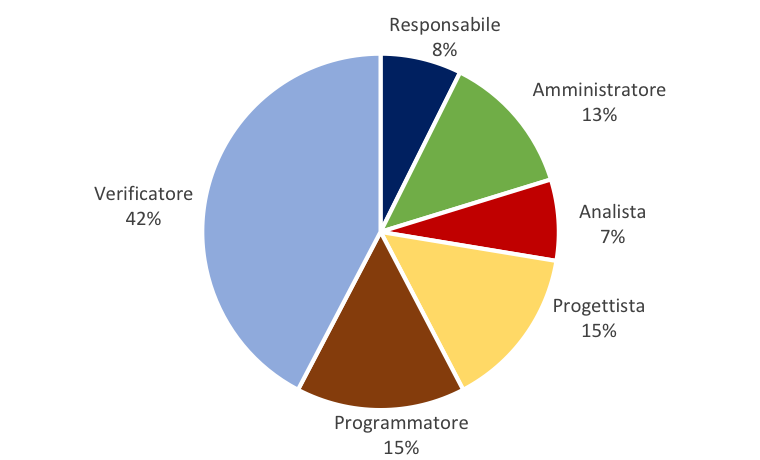
\includegraphics{images/grafoValidazioneCollaudoEuro.png}
		\caption{Grafico prospetto economico nel periodo di Validazione e Collaudo}
	\end{center}
\end{figure}
\newpage
\section{Totale ore rendicontate}
\subsection{Totale del  prospetto orario rendicontato}
Il totale del prospetto orario rendicontato è illustrato nella seguente tabella:

\begin{table}[ht]
	\begin{center}
		\rowcolors{1}{}{lightgray}
		\begin{tabular}{ccccccccc}
			\rowcolor{coolblack}
			\hline
			& \textcolor{white}{Nome} & \textcolor{white}{Re} & \textcolor{white}{Am} & \textcolor{white}{An} & \textcolor{white}{Pt} &\textcolor{white}{Pr} & \textcolor{white}{Ve} & \textcolor{white}{Totale} \\
			\hline
			&Mirko Franco & - & 3 & 13 & 28& 27 & 33 & 104  \\
			&Bianca Andreea Ciuche & 5& 6& 6 & 36 & 21& 30 &104 \\
			&Stefano Zanatta & -& 8& 10 & 38 & 22 & 26 & 104 \\
			&Andrea Deidda &  6& - & 9 &35 & 24 & 30 & 104\\
			&Ludovico Brocca & 8& 14 & 3 & 30 & 24 & 25 & 104 \\
			&Matteo Depascale & 6& 8& 4 & 34& 24& 28& 104\\
			&Gian Marco Bratzu & 7& 4 & 2 & 41 & 32 & 18 &104\\
			\hline
			&\textbf{Ore totali ruolo} & 32& 43 & 47 & 242 & 174 & 190 & 728 \\
		\end{tabular}
		\caption{Prospetto orario totale delle ore rendicontate}
	\end{center}
\end{table}


Il seguente grafico mostra una rappresentazione visiva della suddivisione oraria dei ruoli all'interno del gruppo:
\begin{figure}[!ht]
	\begin{center}
		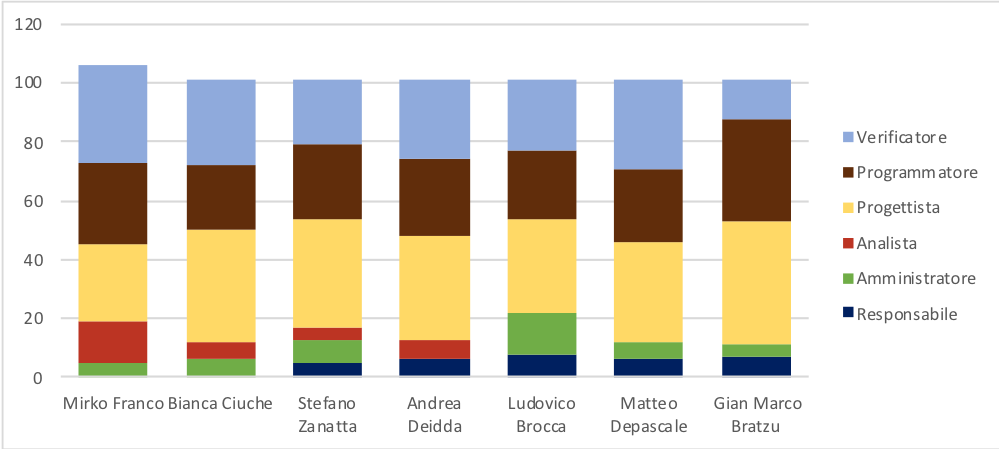
\includegraphics[scale=0.90]{images/grafoOreRendicontate.png}
		\caption{Grafico prospetto orario totale delle ore rendicontate}
	\end{center}
\end{figure}

\subsection{Totale del prospetto economico rendicontato}
La seguente tabella mostra il totale del prospetto economico rendicontato che  include le ore rendicontate nel preventivo a carico del committente cioè dei periodi di Revisione Analisi, Progettazione della Base Tecnologica, Progettazione di Dettaglio e Codifica e il periodo di Validazione e Collaudo.

\begin{table}[ht]
	\begin{center}
		\rowcolors{1}{}{lightgray}
		\begin{tabular}{cccccc}
			\rowcolor{coolblack}
			\hline
			&\textcolor{white}{Ruolo}&	\textcolor{white}{Ore} &\textcolor{white}{Costo(\euro)} \\
			\hline
			&Responsabile           &32&960\\
			&Amministratore        & 43& 860 \\
			&Analista                   & 47& 1.175\\
			&Progettista              &  242& 5.324\\
			&Programmatore       & 174& 2.610 \\
			&Verificatore             & 190& 2.850\\
			\hline
			&\textbf{Ore totali}    &728&13.779\\
		\end{tabular}
		\caption{Prospetto economico totale delle ore rendicontate}
	\end{center}
\end{table}

La raffigurazione grafica del peso di ogni ruolo sul costo totale è così rappresentata:

\begin{figure}[!ht]
	\begin{center}
		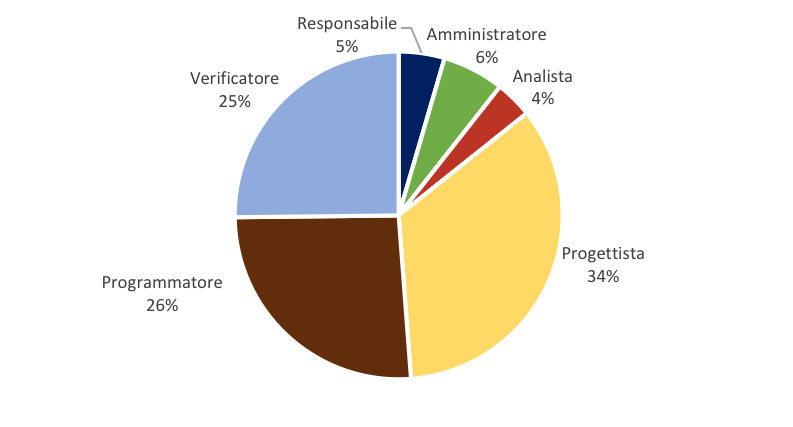
\includegraphics[scale=0.90]{images/grafoOreRendicontateEuro.png}
		\caption{Grafico prospetto economico totale delle ore rendicontate}
	\end{center}
\end{figure}

\section{Totale ore con investimento}
\subsection{Totale del prospetto orario con investimento}
Il totale del prospetto orario con investimento include sia le ore rendicontate nel preventivo a carico del committente sia le ore di investimento iniziali, esso è illustrato nella seguente tabella:

\begin{table}[ht]
	\begin{center}
		\rowcolors{1}{}{lightgray}
		\begin{tabular}{ccccccccc}
			\rowcolor{coolblack}
			\hline
			& \textcolor{white}{Nome} & \textcolor{white}{Re} & \textcolor{white}{Am} & \textcolor{white}{An} & \textcolor{white}{Pt} &\textcolor{white}{Pr} & \textcolor{white}{Ve} & \textcolor{white}{Totale} \\
			\hline
			&Mirko Franco & 10 & 3 & 22 & 28& 27 & 38 & 128  \\
			&Bianca Andreea Ciuche & 5& 12& 16& 36 & 21& 38 &128 \\
			&Stefano Zanatta & 12 & 16& 14 & 38 & 22 & 26 & 128\\
			&Andrea Deidda &  6& 9 & 17 &35 & 24 & 37 & 128\\
			&Ludovico Brocca & 8& 18 & 12 & 30 & 24 & 36 & 128 \\
			&Matteo Depascale & 6& 14& 14& 34& 24& 36& 128\\
			&Gian Marco Bratzu & 7& 10 & 10 & 41 & 32 & 28 &128 \\
			\hline
			&\textbf{Ore totali ruolo} & 54& 82 & 105 & 242 & 174 & 239 & 896 \\
		\end{tabular}
		\caption{Prospetto orario totale delle ore di investimento e rendicontate}
	\end{center}
\end{table}

Il seguente grafico mostra una rappresentazione visiva della suddivisione oraria dei ruoli all'interno del gruppo:
\begin{figure}[!ht]
	\begin{center}
		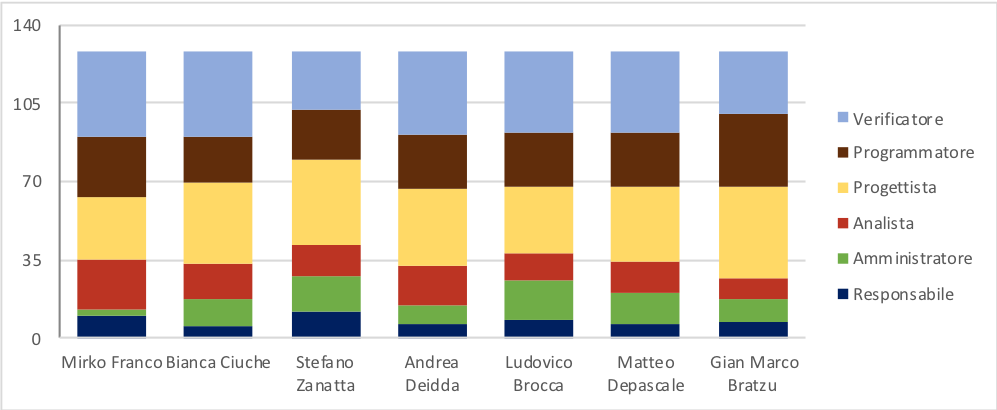
\includegraphics[scale=0.80]{images/grafoOreInvestimento.png}
		\caption{Grafico prospetto orario totale delle ore di investimento e rendicontate}
	\end{center}
\end{figure}
\newpage
\subsection{Totale del prospetto economico con investimento}
Il totale del prospetto economico con investimento include sia le ore rendicontate nel preventivo a carico del committente sia  le ore  di investimento iniziali, esso è illustrato nella seguente tabella:

\begin{table}[ht]
	\begin{center}
		\rowcolors{1}{}{lightgray}
		\begin{tabular}{cccccc}
			\rowcolor{coolblack}
			\hline
			&\textcolor{white}{Ruolo}&	\textcolor{white}{Ore} &\textcolor{white}{Costo(\euro)} \\
			\hline
			&Responsabile           &54&1.620\\
			&Amministratore        & 82& 1.640 \\
			&Analista                   & 105& 2.625\\
			&Progettista              &  242& 5.324\\
			&Programmatore       & 174& 2.610 \\
			&Verificatore             & 239& 3.585\\
			\hline
			&\textbf{Ore totali}    &896&17.404\\
		\end{tabular}
		\caption{Prospetto economico totale delle ore di investimento e rendicontate }
	\end{center}
\end{table}

La raffigurazione grafica del peso di ogni ruolo sul costo totale è così rappresentata:
\begin{figure}[!ht]
	\begin{center}
		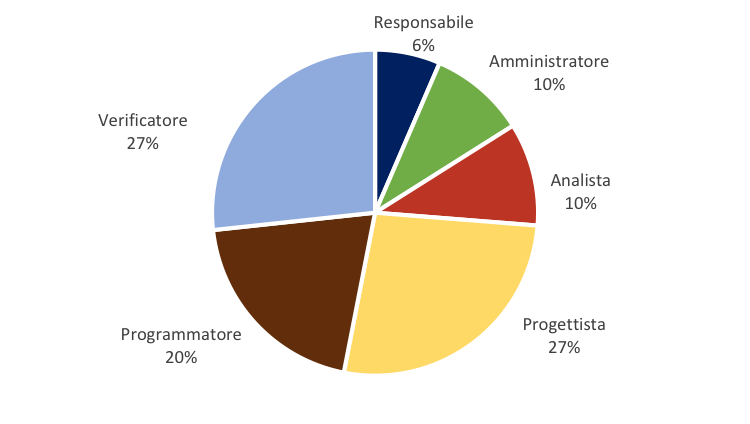
\includegraphics[scale=0.90]{images/grafoOreInvestimentoEuro.png}
		\caption{Grafico prospetto economico totale delle ore di investimento e rendicontate}
	\end{center}
\end{figure}